\documentclass[10pt]{beamer}
\beamertemplatenavigationsymbolsempty

\usepackage[utf8]{inputenc}
\usepackage{default}

\usepackage{graphicx}
\graphicspath{{pictures/}}

\usepackage[french]{babel}
\usepackage[T1]{fontenc}

\usetheme{metropolis}
%\usecolortheme{dove}

\begin{document}

\begin{frame}
\frametitle{Université de Technologie de Belfort-Montbéliard\\
            Département informatique}
\begin{center}
    {\LARGE Projet IN55}\\
    \vskip 1em
    {\Large Animation d'un personnage 3D}
\end{center}
\vskip 1em
\begin{flushright}
    Responsable: Fabrice Lauri
\end{flushright}
Florent \textsc{Jacquet}\\
Romain \textsc{Thibaud}\\
Antonin \textsc{WALTZ}\\
{\scriptsize IN55 - A15}
\end{frame}

\begin{frame}
 	\frametitle{Sommaire}
	\tableofcontents
\end{frame}

\section{Modélisation}
\begin{frame}
\frametitle{Modélisation}
\begin{itemize}
    \item Utilisation de Blender
    \item 3 animations : marcher, s'asseoir, voler
\end{itemize}
\begin{figure}[htpb]
    \centering
    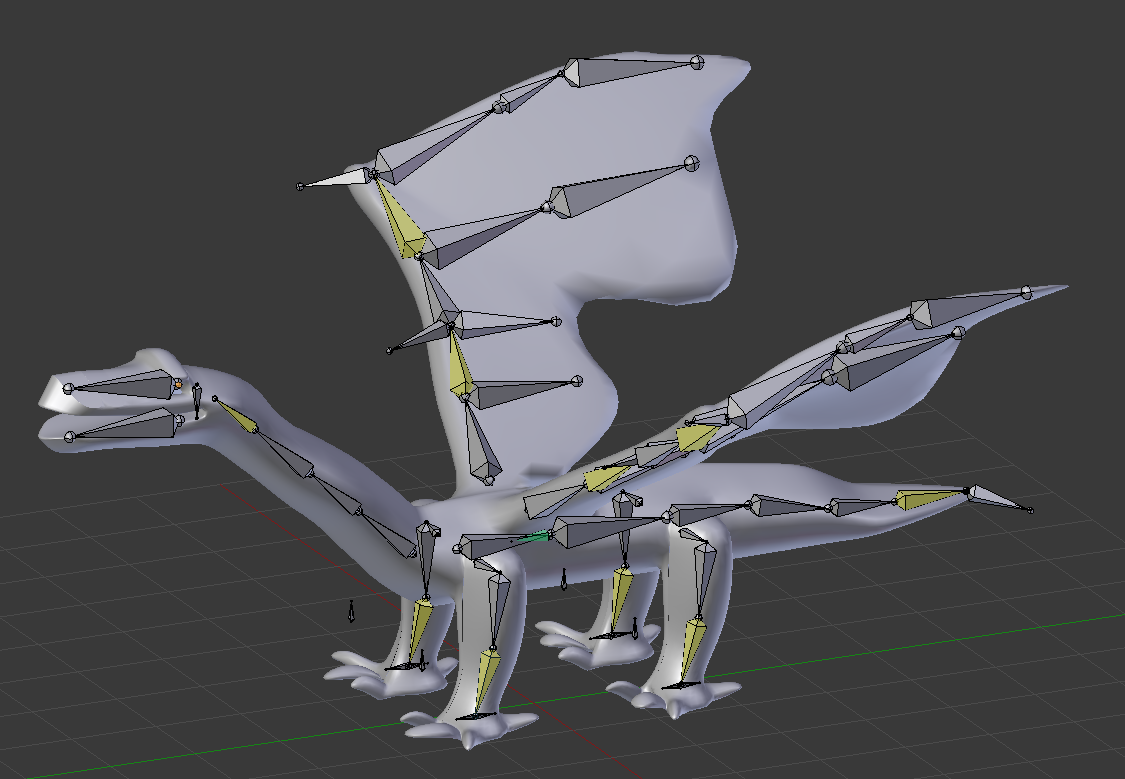
\includegraphics[width=0.7\linewidth]{armature.png}
    \caption{Modèle du dragon avec son armature}
\end{figure}
\end{frame}

\section{Choix technologiques}
\begin{frame}
\frametitle{Choix technologiques}
\begin{itemize}
    \item Utilisation de la librairie Asset Import
    \item %TODO
\end{itemize}
\end{frame}

\section{Architecture}
\begin{frame}
\frametitle{Structure d'un Mesh}
\begin{figure}[H]
    \begin{center}
        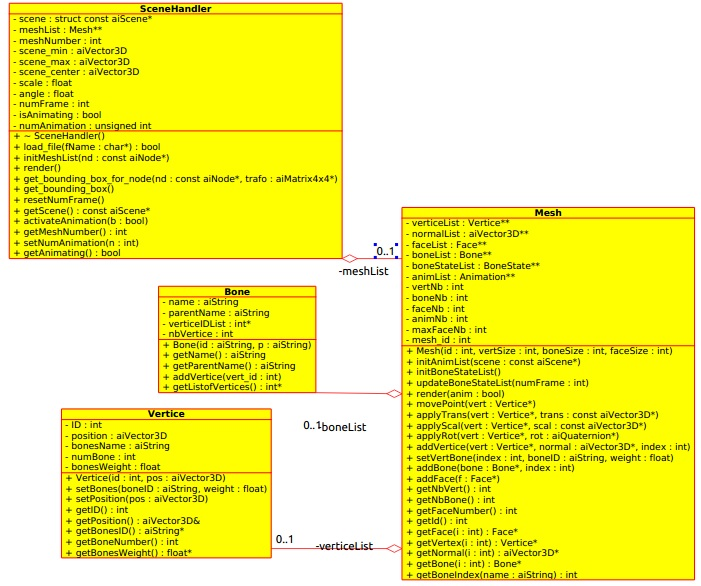
\includegraphics[width=0.7\textwidth]{MeshStructure.jpg}
        \caption{Diagramme de classe pour la structure d'un Mesh}
    \end{center}
\end{figure}
\end{frame}

\begin{frame}
\frametitle{Structure d'une Animation}
\begin{figure}[H]
    \begin{center}
        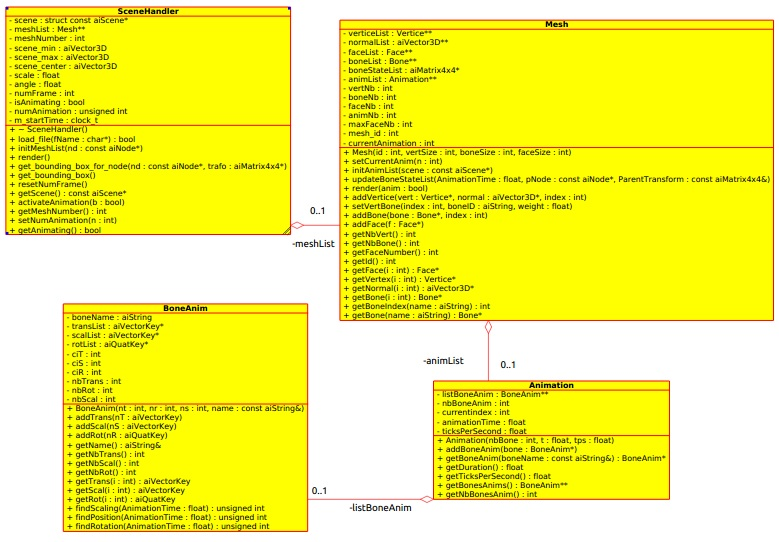
\includegraphics[width=0.7\textwidth]{AnimStructure.jpg}
        \caption{Diagramme de classe pour la structure d'une animation}
    \end{center}
\end{figure}
\end{frame}


\section{Bilan}
\begin{frame}
\frametitle{Difficultés rencontrées}
\begin{itemize}
	\item Prise en main des Inverse Kinematics et de Blender en général
	\item Prise en main de la librairie Assimp
	\item Comprendre comment parcourir de grandes quantités de données à travers des structures complexes pleines de références croisées
	\item Gestion de la mémoire en C++
\end{itemize}
\end{frame}

\begin{frame}
\frametitle{Améliorations}
\begin{itemize}
	\item Texturer le modèle
	\item Intégrer un système de gestion de la lumière
	\item Améliorer la fluidité et le maniement de la caméra libre
\end{itemize}
\end{frame}

\begin{frame}
\frametitle{Conclusion}
\begin{itemize}
	\item Première expérience de programmation graphique avec OpenGL
	\item Découverte de la librairie Asset Import
\end{itemize}
\end{frame}

\begin{frame}
\begin{center}
\textbf{Merci de votre attention}\\
    Questions?\\
    Remarques?\\
\end{center}
\end{frame}

\end{document}
